%!TEX root = ../document-diss.tex

\chapter{Konditionale Operatoren.} 
Das sind Boole’sche Operatoren, die eine Menge Spaß machen

\section{Widmung}


\toggletrue{hund}

Diese Doktorarbeit widme ich von Herzen 
\iftoggle{hund}%Abfrage
{meinem Hund.}%true
{meinen lieben Eltern.}%false

\togglefalse{hund}

Diese Doktorarbeit widme ich von Herzen 
\iftoggle{hund}%Abfrage
{meinem Hund.}%true
{meinen lieben Eltern.}.%false

%---
%  Folgendes Szenario: In der offiziellen Abgabeversion möchte ich meinen Eltern danken. 
%  Aber ein Extraexemplar soll meinem Hund gewidmet sein.
% Kann man das machen, dass man das irgendwie automatisch ändern kann?
%---


\section{Abbildungen}

\subsection{Die zwei Brüder von Humboldt}

%--------------------------------
% Jetzt wird es schwierig: Die zwei Brüder sollen nebeneinander gesetzt werden.
% alexander.jpg und wilhelm.jpg
% Als Bildunterschrift: Alexander von Humboldt // Wilhelm von Humboldt
% Als gemeinsame  Bildunterschrift: Die Brüder von Humboldt
% Die Bilder bitte gleich hoch setzen.
%-------------------------------
\begin{figure}[h]
	{\missingcopyright
	\subcaptionbox{%
		Alexander von Humboldt}{%
		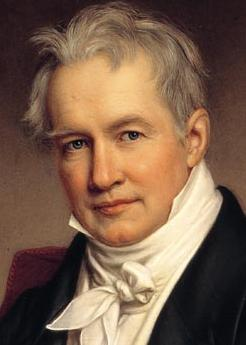
\includegraphics[height=5cm]{figures/alexander}}%hier draft einfügen in eckigen Klammern -> damit das ausgebelnedet
	}
	\hfil%hspace*{3cm}
	\subcaptionbox{%
	Wilhelm von Humboldt}{%
	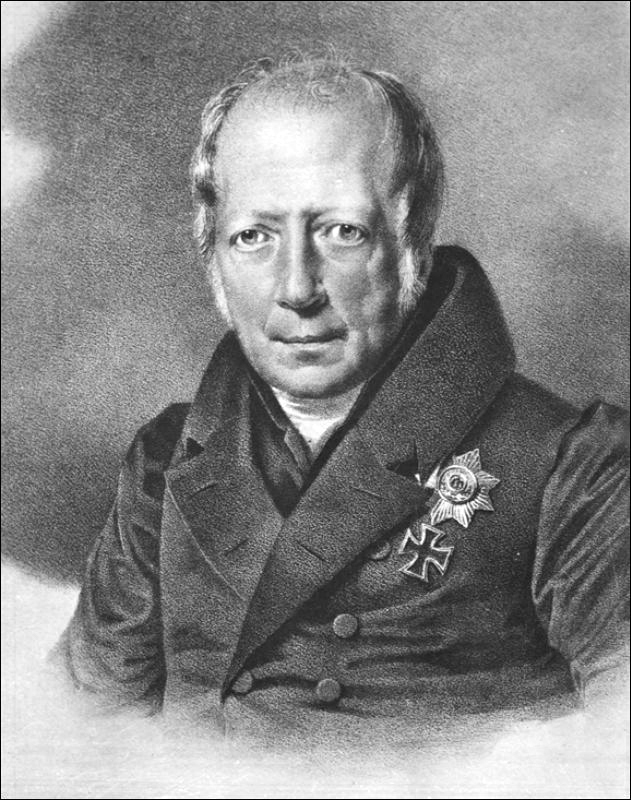
\includegraphics[height=5cm]{figures/wilhelm}}
	\caption{Die Brüder von Humboldt}
\end{figure}

%---
% Ich habe allerdings nur für Wilhelm die Druckgenehmigung bekommen,
% nicht für Alexander.
% Das heißt, dass in meiner Abgabeversion beide Bilder zusehen sein müssen,
% in der finalen Printfassung muss Alexander ausgeblendet werden.
% Die Maße und die Bildunterschrift sollen erhalten bleiben
% und nur das Bild mit einem Platzhaltertext versehen werden.
%---







